%\documentclass[aps,prl,twocolumn,showpacs,superscriptaddress,groupedaddress]{revtex4}
%% for review and submission
%\documentclass[aps,preprint,showpacs,superscriptaddress,groupedaddress]{revtex4}
% for double-spaced preprint
%\documentclass[aps,prl,floatfix,twocolumn,10pt]{revtex4-1}
%for review and submission
%\documentclass[aps,prl,preprint]{revtex4-1} 
% for double-spaced preprint
%\documentclass[aip,apl,amsmath,amssymb,floatfix,preprint,a4paper]{revtex4-1}
\documentclass[aip,apl,amsmath,amssymb,floatfix,reprint,a4paper]{revtex4-1}

%% Packages
\usepackage[utf8]{inputenc} %Umlaute
\usepackage{acronym}
\usepackage{amsmath}
\usepackage{amssymb}
\usepackage{graphicx}  %figures
\usepackage[detect-all]{siunitx}

%% New commands
\newcommand{\msub}[1]{\ensuremath{\textnormal{\begin{tiny}#1\end{tiny}}}}
\renewcommand{\d}[1]{\ensuremath{\operatorname{d}\!{#1}}}

%acronyms
\acrodef{CT}{computed tomography}
\acrodef{SNR}{signal-to-noise ratio}
\acrodef{CNR}{contrast-to-noise ratio}
%% ----------------------------------------------------------------------------------------------------------------

\begin{document}

\title{X-ray phase-contrast imaging at \SI{100}{\kilo\electronvolt}}

\author{T.~Thüring}
\affiliation{Paul Scherrer Institut, Villigen PSI, Switzerland}
\affiliation{Institute for Biomedical Engineering, Swiss Federal Institute of Technology, Zurich, Switzerland}
\author{M.~Abis}
\affiliation{Paul Scherrer Institut, Villigen PSI, Switzerland}
\affiliation{Institute for Biomedical Engineering, Swiss Federal Institute of Technology, Zurich, Switzerland}
\author{Z.~Wang}
\affiliation{Paul Scherrer Institut, Villigen PSI, Switzerland}
\author{C.~David}
\affiliation{Paul Scherrer Institut, Villigen PSI, Switzerland}
\author{M.~Stampanoni}
\affiliation{Paul Scherrer Institut, Villigen PSI, Switzerland}
\affiliation{Institute for Biomedical Engineering, Swiss Federal Institute of Technology, Zurich, Switzerland}

\date{\today}


%% ----------------------------------------------------------------------------------------------------------------
\begin{abstract}
    Phase contrast imaging with X-rays provides access to
    complementary physical contrast mechanisms. Phase sensitive imaging in
    the diagnostic energy range between $80$ and
    $\SI{150}{\kilo\electronvolt}$ is still largely unexplored, as the
    current methods typically entail severe technical challenges. A
    phase-contrast technique at such high energies is of scientific and
    industrial interest as it vastly expands the range of applications, for
    instance, by the examination of materials of high density or thickness.
    The approach includes a new design for the grating manufacturing in
    Talbot-Lau interferometry, with an edge-on illumination and curved
    structures to match the beam divergence. The edge-on approach breaks the
    current limits of achievable grating aspect ratios, which has been a key
    issue for a long time. The curvature of the gratings solves the
    intrinsic reduction of the field of view which occurs for gratings with
    such high aspect ratios. Using an imaging arrangement based on a
    conventional X-ray tube, phase and dark-field contrast imaging at
    $\SI{100}{\kilo\electronvolt}$ is demonstrated. This achievement paves
    the road for the transfer of phase-contrast imaging into fields where
    high energies are required, such as medical computed tomography, chip
    failure analysis or homeland security.
\end{abstract}

\maketitle

%%%%%%%%%%%%%%%%%%%%%%%%%%%%%%%%%%%%%%%%%%%%%%%%%%%%%%%%%%%%%%%%%%%%%%%%
% Body of manuscript
%%%%%%%%%%%%%%%%%%%%%%%%%%%%%%%%%%%%%%%%%%%%%%%%%%%%%%%%%%%%%%%%%%%%%%%%

X-ray radiography and \ac{CT} are nowadays standard imaging techniques in
materials and life sciences for the nondestructive examination of samples or
the diagnosis of diseases in patients. The underlying contrast mechanism
relies on the different X-ray attenuation properties of different materials
or tissue types. The dominant physical effects contributing to attenuation
are the photoelectric effect and incoherent (Compton) scattering. The sum of
their contributions determines the attenuation coefficient, which is a
wavelength dependent material parameter. Besides attenuation, the wave
nature of X-rays reveals another contrast mechanism, which is the phase
shift. The interaction contributing to phase shifts is coherent (Rayleigh)
scattering \cite{Als-Nielsen2011}.

Using the material parameter $n=1-\delta(\mathbf{r},\lambda) + i
\beta(\mathbf{r},\lambda)$, known from X-ray wave optics as the complex
index of refraction, the wavelength dependent attenuation and phase shift
properties of an object at the spatial coordinate $\mathbf{r}$ are fully
described. The imaginary part $\beta(\mathbf{r},\lambda)$ is related to the
attenuation per unit length (attenuation coefficient) by $\mu = 4 \pi
\beta(\mathbf{r},\lambda) / \lambda$ and the total attenuation by an object
of thickness $d$ can be described by the line integral $L_\mu = \int_0^d
\mu(\mathbf{r},\lambda) \d l$. Similarly, the real part
$\delta(\mathbf{r},\lambda)$ determines the phase shift per unit length by
$\phi = 2 \pi \delta / \lambda$ and the total phase shift is $L_\phi =
\int_0^d \phi(\mathbf{r}) \d l$.

While the attenuation line integral $L_\mu$ can be directly measured with an
X-ray detector by measuring the reduction of the beam intensity $I$ ($L_\mu
\propto \log(I)$), the measurement of the phase shift integral $L_\phi$ is
more challenging as there is no such simple relation. However, phase
sensitive imaging is a desirable modality, as it can provide an enhanced
\ac{CNR} in images compared to attenuation for certain
materials or in different tissues \cite{Pfeiffer2007a,McDonald2009}.
Furthermore, the refractive index decrement $\delta$ provides direct access
to the electron density \cite{Als-Nielsen2011} and in combination with
attenuation, it further enables the determination of the effective atomic
number of a material \cite{Qi2010}.

In the past, a lot of effort has been invested into the development of
techniques which are sensitive to the phase shift. Since most of the
available phase contrast techniques rely on interference and thus typically
on optical hardware (e.g. crystals, gratings), they vary a lot in terms of
sensitivity, practical applicability or achievable resolution. The vast
majority of the methods, including crystal analyzer based
\cite{Davis1995,Chapman1997} or interferometric \cite{Bonse1965,Momose1996}
methods rely on X-ray beams of high spatial and temporal coherence, which is
available only at synchrotron sources. Techniques which are compatible with
an X-ray beam of low temporal coherence (broad bandwidth) are the in-line
phase contrast method \cite{Snigirev1995,Wilkins1996,Cloetens1996} and
Talbot interferometry \cite{Cloetens1997,David2002,Momose2003a}.
Phase-contrast imaging using X-ray beams of low temporal \emph{and}
spatial coherence such as conventional low-brilliance X-ray tubes have been
demonstrated with Talbot-Lau interferometry \cite{Pfeiffer2006} and coded
apertures \cite{Munro2012}.

Phase-contrast imaging has so far been used in the energy
range from $15$ up to $\SI{85}{\kilo\electronvolt}$. Talbot
interferometry has been demonstrated using a synchrotron source at
$\SI{82}{\kilo\electronvolt}$ \cite{Willner2013}. Also using a synchrotron
source, phase-contrast imaging at $\SI{85}{\kilo\electronvolt}$ has been
reported. Using a low-brilliance X-ray tube, Talbot-Lau interferometry was
applied at $\SI{60}{\kilo\electronvolt}$ mean energy \cite{Donath2009}.
Medical imaging applications may benefit from phase contrast at higher
energies: chest or abdominal
radiography or \ac{CT} require energies between $100$ and
$\SI{150}{\kilo\electronvolt}$. Other potential applications are homeland
security or chip failure analysis, which require high energies for the
visualization of materials of high density and atomic number.

Here, we introduce a method for phase-contrast imaging which is
compatible with the entire diagnostic energy range of X-rays. Moreover, the
method is fully compatible with compact imaging arrangements based on
conventional X-ray tubes. The method is based on Talbot-Lau interferometry
\cite{Pfeiffer2006} and employs an edge-on approach for the grating design and
arrangement. Up to now, Talbot-Lau interferometry has been applied with a
maximum design energy of $\SI{60}{\kilo\electronvolt}$ \cite{Donath2009}.
The challenge which limited the progress towards higher energies was mainly
related to the manufacturing of gratings with high aspect ratios. The aspect
ratio, given by
\begin{equation}
    \text{AR} = \frac{2h}{p},
\end{equation}
where $p$ is the grating period and $h$ the grating structure
height, is normally limited by the lithographic process, as grating
structures tend to collapse or to deform (e.g. through capillary forces) if
the aspect ratio is too high. For a given setup distance these parameters
depend on the target energy $E$ according to $p \propto
1/\sqrt{E}$ and $h \propto E^3$, and therefore $\textnormal{AR}
\propto E^{7/2}$\cite{Momose2003a}. If at $E=\SI{25}{\kilo\electronvolt}$ an aspect ratio
for the absorption grating of around $\textnormal{AR}=30$ is necessary for a
reasonable length of the experimental arrangement, it would have to be at
least $128$ for $E=\SI{100}{\kilo\electronvolt}$. Moreover, when using a
broad spectrum, photons above the design energy should also be
efficiently attenuated by the gratings, which requires even higher aspect ratios.
Maximum achievable aspect ratios of current grating fabrication techniques
\cite{David2007,Kenntner2010} are approximately around 60,
larger values are often not achievable or come at the expense of a very poor
grating quality and performance.

Our design introduces the edge-on
illumination of circularly aligned structures. Edge-on illumination
(figure~\ref{Fig:schematic}), as
opposed to face-on illumination, exploits the dimension along the grating
lines to form a high aspect ratio of the structures in direction of the beam. The
effective structure height of the grating is then determined by the grating
dimension along the grating lines, which essentially allows arbitrarily high
aspect ratios. 
\begin{figure}[ht]
    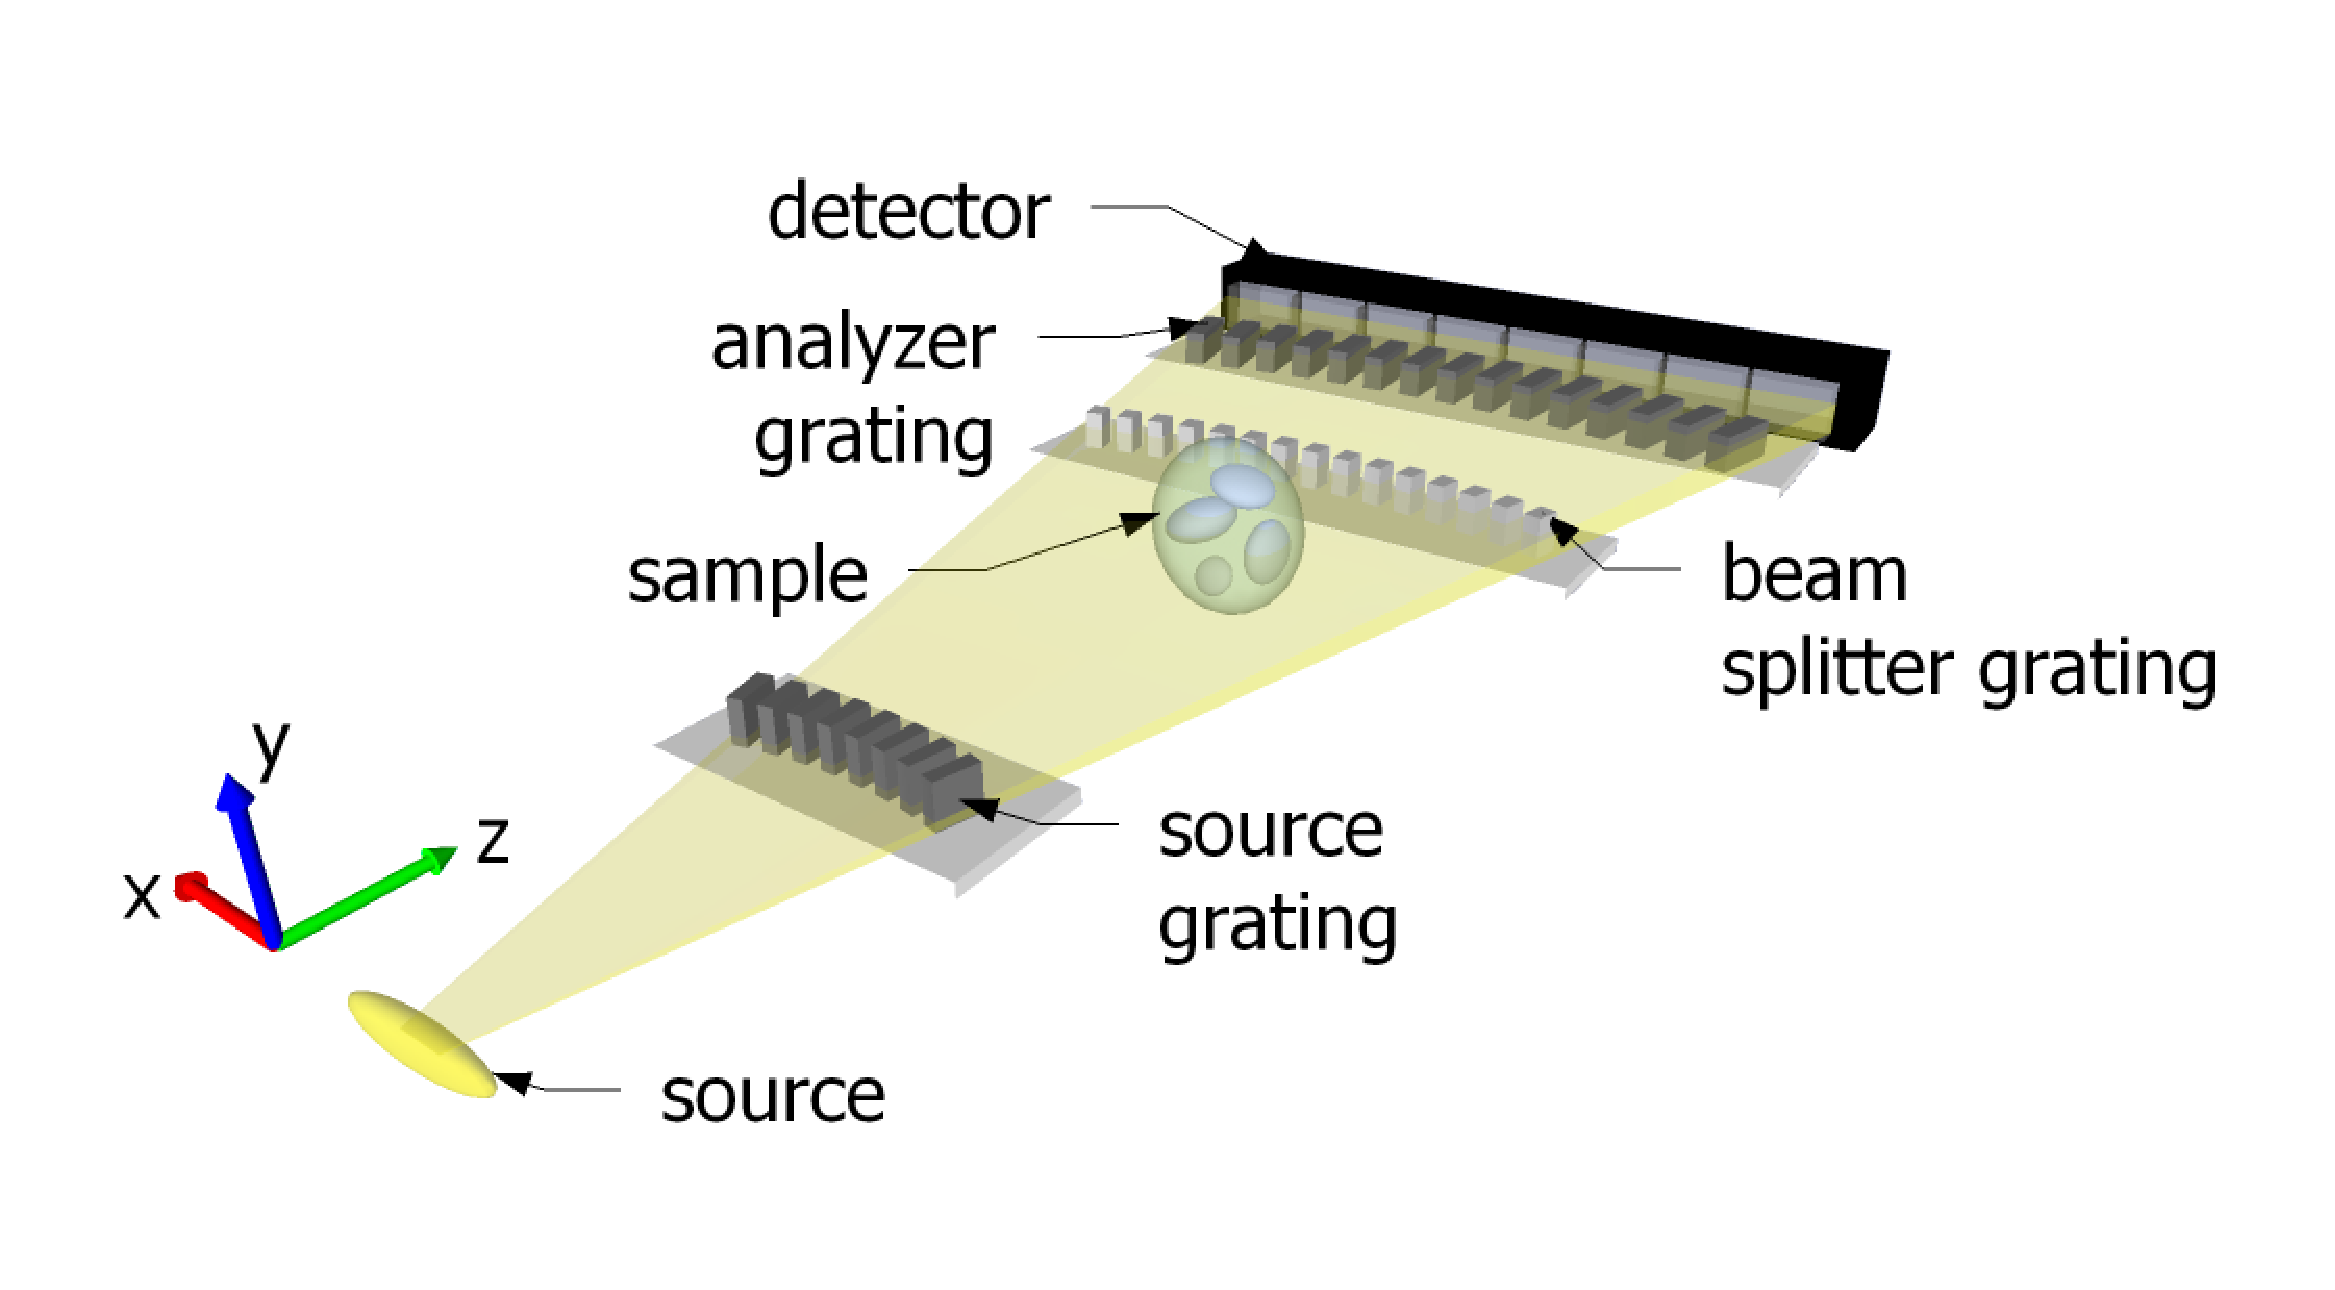
\includegraphics[width=\linewidth]{figures/figure1.eps}
    \caption{Schematic of a grating
        interferometer for X-ray energies between 60 and
        \SI{150}{\kilo\electronvolt} in edge-on illumination mode. The
        aspect ratio is defined by the ratio of the travelling distance along the
        grating lines and the period and can be arbitrarily long. In order to avoid
        a reduction of the field of view, the grating structures are aligned on an
    arc.}
    \label{Fig:schematic}
\end{figure}

Increasing the aspect ratio of the gratings typically leads to a
reduction of the field of view due to the change of the grating transmission
function at high incident angles, which has also been identified by using a
glancing angle of the gratings between zero and \SI{90}{\degree}
\cite{Stutman2012a}. In order to overcome this problem, the grating lines are circularly aligned 
with a radius equal to the distance to the source.

The combination of edge-on illumination and circularly aligned structures
enables phase-contrast imaging at arbitrary design energies and with a
maximum field of view in the horizontal direction ($x$ direction). These
advantages come at the expense of a limited field of view in the vertical
direction ($y$ direction), which is, depending on the X-ray detector,
typically a few pixels. However, radiographic 2D imaging is possible in
scanning mode, without increasing dose. Similarly, for tomographic images,
the approach allows single slice \ac{CT} or full 3D imaging in scanning mode.

Grating design and fabrication is nonstandard and involves a complex mask
design, as shown in Figure~\ref{Fig:grating_mask}. Each grating resides on a
silicon chip and has its specific structure length and curvature. For the
current experiments, a symmetric interferometer with a grating period of $p
= \SI{2.8}{\micro\metre}$ for all gratings has been used. The design energy
is $\SI{100}{\kilo\electronvolt}$ and the beam splitter grating periodically
shifts the phase by zero and $\pi$ at this energy \cite{David2002}. Using
gold as the phase shifting material, this requires a structure length of
$h_1 = \SI{19.8}{\micro \metre}$. The analyzer grating is an absorption mask
for sensing slight changes of the interference pattern generated by the beam
splitter \cite{Momose2003a}. With a structure length of $h_2 =
\SI{800}{\micro \metre}$, this grating has an aspect ratio of $2h/p \approx
570$ and thus sufficiently attenuates X-rays up to energies of 
$\SI{160}{\kilo\electronvolt}$. Beam splitter- and analyzer grating are
separated at the first fractional Talbot order \cite{Weitkamp2005},
resulting in an intergrating distance of $\SI{158}{\milli\metre}$. The
source grating splits the relatively large focal spot ($\sim
\SI{1}{\milli\metre}$) into an array of individually coherent, but mutually
incoherent sources \cite{Pfeiffer2006}. It is also made of gold structures
with a structure length of $h_0 = h_2 = \SI{800}{\micro \metre}$.
\begin{figure} [ht]
    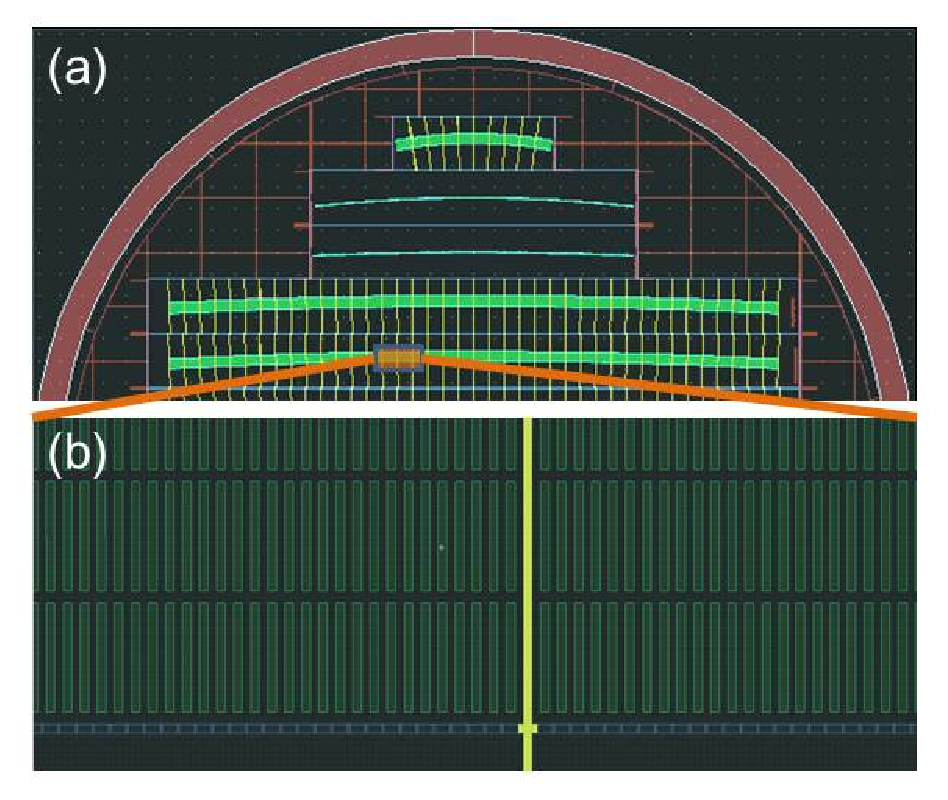
\includegraphics[width=\linewidth]{figures/grating_mask.eps}
    \caption{Grating design mask for
        the edge-on illumination approach. (a) Top part of the 4 inch wafer,
        showing five grating chips; one source grating, two beam splitter
        gratings and two analyzer gratings (from top to bottom). The
        gratings have different curvatures which are specific to the grating
        interferometer geometry. (b) Zoom into the grating structures,
        contain interrupting bridges used for stabilizing the grating
        structures in the lithographic process \cite{Kenntner2010}.}
        \label{Fig:grating_mask}
\end{figure}

Due to the high spectral acceptance \cite{Weitkamp2005,Thuering2013c} of the
interferometer ($\SI{50}{\kilo\electronvolt}$ to
$>\SI{160}{\kilo\electronvolt}$) and the high attenuation efficiencies of
the source- and analyzer gratings ($>90\%$ up to
$\SI{160}{\kilo\electronvolt}$), the voltage of the X-ray source was set to
the maximum of $\SI{160}{\kilo\volt}$. With a grating structure height of
approx. $\SI{100}{\micro \metre}$, the field of view in the vertical
direction is limited to one detector pixel row. In the horizontal direction,
the field of view is limited by the grating size and the geometric
magnification of the sample, yielding a maximum field of view of
$\SI{30}{\milli\metre}$. In addition to the standard components (source,
camera, interferometer), two optical slits, one in front of the source
grating, the other in front of the camera, were required for the collimation
of the beam in the vertical direction. X-rays which are not travelling
through all of the gratings do not contribute to the signal and are
attenuated by the slits.

%Fig. 3 shows a radiographic image of a metal screw in all three contrast
%modes, acquired with the $\SI{100}{\kilo\electronvolt}$ setup. The images
%were acquired in scanning mode, using a step size of $\SI{100}{\micro
%\metre}$. The number of phase steps was 24 and the exposure time was 15
%seconds per step. Grating interferometry at such a high diagnostic energy
%allows to examine more dense materials such as metals in phase contrast
%mode. At lower energies, the phase shifts of such materials would be too
%large and wrap over multiple periods of the analyzer grating.

Fig.~\ref{Fig:img_chip} shows a radiographic scan of an electronic chip.
Several resistors and an integrated circuits are located on different layers
on the chip. The images were acquired in scanning mode, using a step size of
$\SI{100}{\micro \metre}$ along the $y$ axis. For a better comparison of the
magnified phase and attenuation images, the attenuation image has been
replaced with the differential attenuation image, which was obtained by
digital differentiation. In the attenuation image, the soldering points of
the integrated circuit are hardly visible underneath the resistors, while in
the phase image, they can clearly be identified. This shows the
benefit of the differential nature of the phase-contrast image, which may be
useful to identify flaws in multi-layered structures such as electronic
chips.
\begin{figure}[ht]
    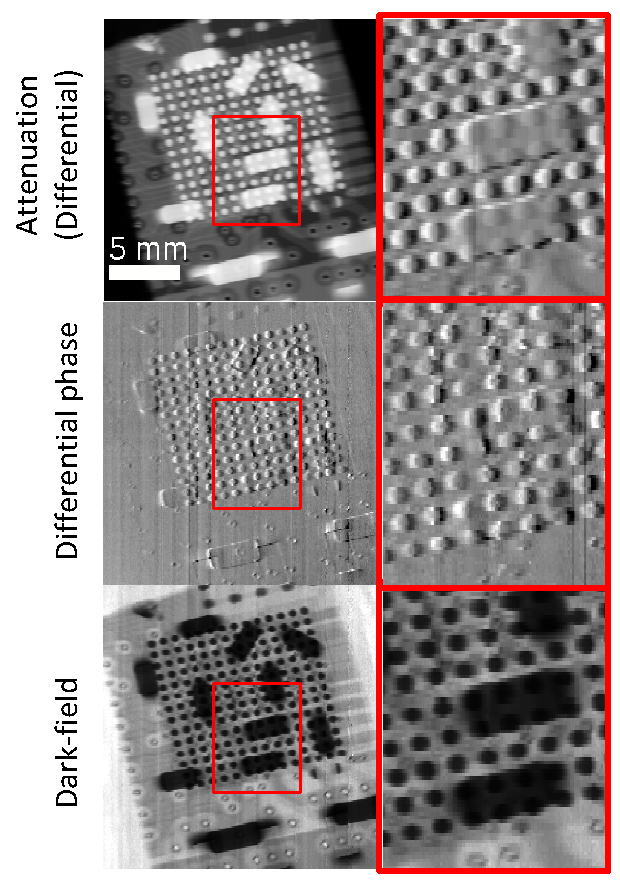
\includegraphics[width=\linewidth]{figures/img_chip_dabs.eps}
    \caption{Radiographic scan of an electronic chip. The image was acquired
        with 24 phase steps and an exposure time of \SI{15}{\second} per
    step.}
    \label{Fig:img_chip}
\end{figure}

Edge-on illuminated grating interferometry breaks the current limitations of
phase-contrast imaging to the lower diagnostic energy range. Compact
geometries  using conventional X-ray sources for design energies well above
$\SI{100}{\kilo\electronvolt}$ could be realized with the approach. This
enables the examination of materials of higher density or thickness which
would be intransparent at lower energies. Finally, the approach is not
limited to X-ray imaging, but could easily be applied to other grating-based
imaging modalities (e.g., with neutrons \cite{Grunzweig2008}) where high
aspect ratios are required.

\section*{Methods}
Edge-on illuminated gratings were manufactured by Micro
Works GmbH, Germany, using a LIGA process \cite{Kenntner2010}. Each grating
resides on a $5 \times \SI{60}{\milli\metre^2}$ silicon chip and several
grating chips are fabricated on a single 4 inch silicon wafer. The
experimental arrangement for a design energy at \SI{100}{\kilo\electronvolt}
is a symmetric Talbot-Lau interferometer with a grating period of $p =
\SI{2.8}{\micro \metre}$ for all gratings. The distance from the source
grating to the analyzer grating is $\SI{32}{\centi\metre}$ and the source
grating is positioned $\SI{23}{\centi\metre}$ away from the source. The
number of phase steps for one projection was 24 \cite{Weitkamp2005} and the
exposure time for the images was 15 seconds per phase step.

The X-ray source is a COMET MXR-160HP/11 X-ray tube with a maximum output
voltage of $\SI{160}{\kilo\volt}$. In the experiment, it was set to the
maximum voltage. The focal spot size is approximately
$\SI{1}{\milli\metre}$. The detector is a CCD camera from Finger Lakes
Instruments. A cesium iodide (CsI:Ti) scintillator of $\SI{600}{\micro
\metre}$ thickness converts the X-rays to visible light and is coupled with
an optical lens projecting the image onto the CCD. The effective pixel size
is $\SI{80}{\micro \metre}$. The widths of the collimating slits are
$\SI{25}{\micro \metre}$ and $\SI{100}{\micro \metre}$, respectively.

In Fig.~\ref{Fig:img_chip}, image acquisition involved 24 phase steps
\cite{Weitkamp2005} and an exposure time of 15 seconds per step.

\section*{Acknowledgements} We thank Gordan Mikuljan from Paul Scherrer
Institute, Switzerland, for his work on the mechanical design, Joachim
Schulz and Marco Walter from Micro Works GmbH, Germany, for the competent
support on grating design issues, Christian Kottler and Vincent Revol from
Centre Suisse d'Electronique et de Microtechnique (CSEM), Switzerland for
the fruitful discussions on the design of the system.

\bibliographystyle{apsrev4-1} \bibliography{library}

\end{document}
